\section{a) A rendszer modellje és az átviteli függvény ($i_g \to \Omega_2$)}

\subsection{Modellalkotás és struktúragráf}
A rendszer elektromos részében egy ideális áramgenerátor ($i_g$) táplálja a DC motort. Mivel az áramgenerátor a kör áramát egyértelműen meghatározza, a motor tekercsének $R$ ellenállása és $L$ induktivitása nem befolyásolja a motor által kifejtett nyomatékot. A motor által szolgáltatott mechanikai nyomaték:
\begin{equation}
	M_m(t) = k_m i_g(t)
\end{equation}

A mechanikai oldalon a hajtáslánc két tárcsából áll, amelyeket egy rugalmatlan szíj köt össze. A szíj kinematikai kényszert jelent a két tárcsa szögsebessége között:
\begin{equation}
	v = r_1 \Omega_1 = r_2 \Omega_2 \implies \Omega_1 = \frac{r_2}{r_1} \Omega_2
\end{equation}
A hajtáslánc tehát egy ideális transzformátorként modellezhető, melynek áttétele $N = \frac{r_2}{r_1}$.

A rendszer struktúragráfja a mobilitási (erő-áram) analógia alapján az alábbiak szerint rajzolható fel:

\begin{center}
\begin{tikzpicture}[>=stealth, thick, font=\sffamily,
        midarrow/.style={decoration={markings, mark=at position 0.5 with {\arrow{>}}}, postaction={decorate}}]

    % Ground lines
    \draw[ultra thick] (0,0) -- (4.6,0);
    \node[below] at (2.3, 0) {$U_{\text{ref}}=0$};
    
    \draw[ultra thick] (5.0,0) -- (12.2,0);
    \node[below] at (8.6, 0) {$\Omega_{\text{ref}}=0$};

    % Áramforrás
    \draw[thick, ->] (0.5, 0) -- (0.5, 2.0) node[midway, left] {$i_g$};
    \coordinate (U1) at (0.5, 2.0);
    \fill (U1) circle (2pt) node[above left] {$U_1$};

    % Impedances
    \coordinate (U2) at (2.2, 2.0);
    \coordinate (U3) at (3.9, 2.0);
    \draw[thick, midarrow] (U1) to[out=45, in=135] node[above] {$R$} (U2);
    \fill (U2) circle (2pt) node[below] {$U_2$};
    \draw[thick, midarrow] (U2) to[out=45, in=135] node[above] {$L$} (U3);
    \fill (U3) circle (2pt) node[above right] {$U_3$};

    % km transformer
    \coordinate (km) at (4.8, 1.0);
    \draw[thick] (km) circle (0.7);
    \node at (4.8, 2.1) {$k_m$};
    \draw[thick] (U3) to[out=-30, in=135] (4.3, 1.5);
    \draw[thick] (5.3, 1.5) to[out=45, in=180] (6.2, 2.0);
    \draw[thick, ->] (4.3, 1.5) -- (4.3, 0);
    \draw[thick, ->] (5.3, 1.5) -- (5.3, 0);

    % Node Omega1
    \coordinate (w1) at (6.2, 2.0);
    \fill (w1) circle (2pt) node[above] {$\Omega_1$};

    % J1 and B1
    \draw[thick, ->] (w1) to[out=-110, in=90] (5.9, 1.0);
    \draw[thick, dashed] (5.9, 1.0) -- (5.9, 0);
    \node[left] at (5.9, 0.5) {$J_1$};
    
    \draw[thick, ->] (w1) to[out=-70, in=90] (6.8, 0);
    \node[right] at (6.8, 0.8) {$B_1$};

    % N transformer (Gearbox)
    \coordinate (w1out) at (8.0, 2.0);
    \draw[thick] (w1) -- (w1out);
    
    \coordinate (N) at (8.8, 1.0);
    \draw[thick] (N) circle (0.7);
    \node at (8.8, 2.3) {$N = \frac{r_2}{r_1}$};
    \draw[thick] (w1out) to[out=-30, in=135] (8.3, 1.5);
    \draw[thick] (9.3, 1.5) to[out=45, in=180] (10.2, 2.0);
    \draw[thick, ->] (8.3, 1.5) -- (8.3, 0);
    \draw[thick, ->] (9.3, 1.5) -- (9.3, 0);

    % Node Omega2
    \coordinate (w2) at (10.2, 2.0);
    \fill (w2) circle (2pt) node[above right] {$\Omega_2$};

    % J2 and B2
    \draw[thick, ->] (w2) to[out=-110, in=90] (9.9, 1.0);
    \draw[thick, dashed] (9.9, 1.0) -- (9.9, 0);
    \node[left] at (9.9, 0.5) {$J_2$};
    
    \draw[thick, ->] (w2) to[out=-70, in=90] (11.2, 0);
    \node[right] at (11.2, 0.8) {$B_2$};
\end{tikzpicture}
\end{center}

\subsection{Impedancia-hálózat és redukció}
Mivel a villamos oldalt egy ideális áramgenerátor táplálja, a rendszer az $\Omega_2$ kihajtó tengelyre redukálva felírható egyetlen mechanikai impedancia-hálózatként. Az elektromos oldal és a behajtó tárcsa impedanciáit az áttételek ($k_m$ és $N$) segítségével redukáljuk.

A hajtott ($2$-es) oldalról nézve a bemeneti gerjesztés egy egyenértékű nyomatékforrás:
\begin{equation}
	M'_{be} = M_m \cdot N = k_m i_g \frac{r_2}{r_1}
\end{equation}

A behajtó tárcsa impedanciája ($Z_{mech1} = \frac{1}{J_1 s + B_1}$) a kihajtó tengelyre redukálva:
\begin{equation}
	Z'_{mech1} = \frac{Z_{mech1}}{N^2} = \frac{1}{\left(J_1 \left(\frac{r_2}{r_1}\right)^2\right) s + \left(B_1 \left(\frac{r_2}{r_1}\right)^2\right)}
\end{equation}
Ez azt jelenti, hogy a redukált tehetetlenség $J'_1 = J_1 \left(\frac{r_2}{r_1}\right)^2$, a redukált csillapítás pedig $B'_1 = B_1 \left(\frac{r_2}{r_1}\right)^2$.

A hajtott tárcsa impedanciája:
\begin{equation}
	Z_{mech2} = \frac{1}{J_2 s + B_2}
\end{equation}

A redukált impedancia-hálózat:
\begin{center}
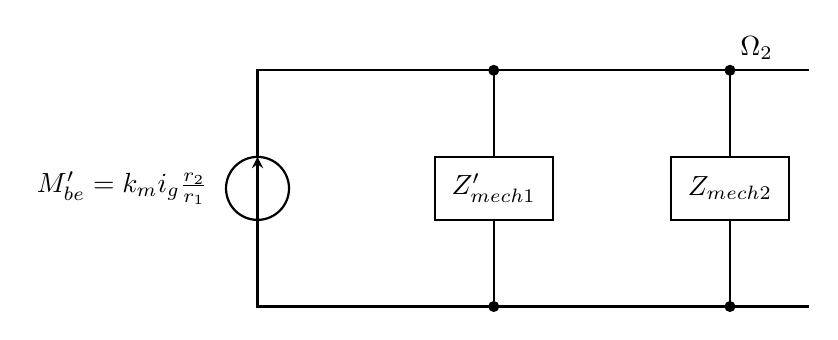
\begin{tikzpicture}[>=stealth, thick,
        block/.style={rectangle, draw, minimum width=1.5cm, minimum height=0.8cm, align=center}
    ]

    % Nyomatékforrás
    \draw[fill=white] (0,1.5) circle (0.4) node[left=0.5cm] {$M'_{be} = k_m i_g \frac{r_2}{r_1}$};
    \draw[->, thick] (0, 1.1) -- (0, 1.9);
    \draw (0,1.9) -- (0,3) -- (1.5,3);
    \draw (0,1.1) -- (0,0) -- (1.5,0);

    % Zmech1'
    \node[block] (Z1) at (3, 1.5) {$Z_{mech1}'$};
    \draw (1.5,3) -- (3,3) -- (Z1.north);
    \draw (1.5,0) -- (3,0) -- (Z1.south);
    \fill (3,3) circle (2pt); \fill (3,0) circle (2pt);

    % Zmech2
    \node[block] (Z2) at (6, 1.5) {$Z_{mech2}$};
    \draw (3,3) -- (6,3) -- (Z2.north);
    \draw (3,0) -- (6,0) -- (Z2.south);
    \fill (6,3) circle (2pt) node[above right] {$\Omega_2$}; \fill (6,0) circle (2pt);
    
    \draw (6,3) -- (7,3);
    \draw (6,0) -- (7,0);
\end{tikzpicture}
\end{center}

\subsection{Az átviteli függvény meghatározása}
A rendszer eredő mechanikai impedanciája az $\Omega_2$ csomópontban a két párhuzamosan kapcsolt impedancia eredője:
\begin{equation}
	\frac{1}{Z_{er}} = \frac{1}{Z'_{mech1}} + \frac{1}{Z_{mech2}} = \left[ J_1 \left(\frac{r_2}{r_1}\right)^2 s + B_1 \left(\frac{r_2}{r_1}\right)^2 \right] + [J_2 s + B_2]
\end{equation}
\begin{equation}
	Z_{er}(s) = \frac{1}{\left[ J_2 + J_1 \left(\frac{r_2}{r_1}\right)^2 \right] s + \left[ B_2 + B_1 \left(\frac{r_2}{r_1}\right)^2 \right]}
\end{equation}

A kimenő szögsebesség a nyomatékforrás és az eredő impedancia szorzata:
\begin{equation}
	\Omega_2(s) = M'_{be}(s) \cdot Z_{er}(s) = k_m I_g(s) \frac{r_2}{r_1} \cdot \frac{1}{\left[ J_2 + J_1 \left(\frac{r_2}{r_1}\right)^2 \right] s + \left[ B_2 + B_1 \left(\frac{r_2}{r_1}\right)^2 \right]}
\end{equation}

Az átviteli függvény ($W_a(s) = \frac{\Omega_2(s)}{I_g(s)}$) kifejezve és időállandós alakba rendezve:
\begin{equation}
	W_a(s) = \frac{\frac{r_2}{r_1} k_m}{\left[ J_2 + J_1 \left(\frac{r_2}{r_1}\right)^2 \right] s + \left[ B_2 + B_1 \left(\frac{r_2}{r_1}\right)^2 \right]}
\end{equation}

A kapott átviteli függvény egy \textbf{arányos egytárolós (PT1)} tag, amelynek erősítése ($A$) és időállandója ($T$):
\begin{equation}
	A = \frac{\frac{r_2}{r_1} k_m}{B_2 + B_1 \left(\frac{r_2}{r_1}\right)^2}, \quad T = \frac{J_2 + J_1 \left(\frac{r_2}{r_1}\right)^2}{B_2 + B_1 \left(\frac{r_2}{r_1}\right)^2}
\end{equation}
